\subsubsection{Running Jupyter Notebooks}

\newline
\href{https://docs.jupyter.org/en/latest/}{Jupyter Notebooks} allow users to display:

\begin{itemize}
\item Interactive and runnable code cells, typically written in \href{https://docs.python.org/3/}{Python}
\item \href{https://jupyter-notebook.readthedocs.io/en/stable/examples/Notebook/Working\%20With\%20Markdown\%20Cells.html}{Markdown} cells containing explanatory text, formulas, hyperlinks, tables, pseudocode, images, etc.
\end{itemize}

Jupyter Notebooks provide an ideal file format for teaching/learning coding concepts and prototyping algorithms.


\bigskip
\centerline{\rule{13cm}{0.4pt}}
\bigskip

\begin{itemize}
\item Notebook~Cell~Types\begin{itemize}
\item Markdown~Cells
\item Code~Cells
\end{itemize}


\item How~to~Run~Jupyter~Notebooks\begin{itemize}
\item Selecting~Cells\begin{itemize}
\item Select~an~Individual~Cell
\item Select~Multiple~Cells
\end{itemize}


\item Hide~Code~Cells\begin{itemize}
\item Collapse~an~Individual~Cell
\item Collapse~Selected~Cells~or~All~Cells~in~a~Notebook
\item Hide~Sections~of~Code~Cells~beneath~a~Markdown~Cell
\end{itemize}


\item Running~Code~Cells\begin{itemize}
\item Run~a~Single~Code~Cell
\item Run~Multiple~Code~Cells\begin{itemize}
\item Run~a~batch~of~selected~cells
\item Run~Every~Cell~Above~or~Below~a~Code~Cel
\item Run~an~Entire~Notebook
\end{itemize}


\item Rerunning~a~Notebook
\end{itemize}


\item Clearing~Cell~Output~Before~Closing
\end{itemize}
\end{itemize}


\bigskip
\centerline{\rule{13cm}{0.4pt}}
\bigskip

\paragraph{Notebook Cell Types}\label{Notebook-Cell-Types}

\subparagraph{Markdown Cells}\label{markdown-cells}

Markdown cells contain documentation in Markdown, MyST Markdown, HTML, and/or LaTeX. They are often used to display text, images, hyperlinks, formulas, tables, pseudocode, plots, figures, etc.

\textbf{Markdown Edit Mode}

To enter edit mode in a markdown cell, double-click the cell.

\begin{figure}[!htbp]
\centering
\includegraphics[width=0.7\linewidth]{files/markdown_cell_edit_m-b8e8c5b3b1cc0a471bb3ae84ec951803.gif}
\caption*{Double-click on a markdown cell to enter edit mode}
\end{figure}

\textbf{Markdown Display Mode}

To render a markdown cell, select it then:

\begin{itemize}
\item Click the \textbf{play} button at the top of the notebook
\end{itemize}

or

\begin{itemize}
\item Use the \texttt{shift + enter} ``play'' shortcut.
\end{itemize}

\begin{figure}[!htbp]
\centering
\includegraphics[width=0.7\linewidth]{files/markdown_run-0dba41b32d4680b49aeb935ccbacf54e.gif}
\caption*{A run markdown cell}
\end{figure}

\subparagraph{Code Cells}\label{code-cells}

Code cells contain editable and runnable Python code. You can run them sequentially or in any order, once or any number of times.

\begin{figure}[!htbp]
\centering
\includegraphics[width=0.7\linewidth]{files/code_cell-626391938035d549c42fc8ffc2ea829b.gif}
\caption*{Selecting and running a code cell}
\end{figure}

\begin{framed}
\textbf{Tip}\\
While the ability to rerun the code cells in arbitrary order can be helpful, it can also cause problems, such as:

\begin{itemize}
\item Recycled variables may contain unexpected values if you run cells in non-sequential order.
\item You may skip cells that set required variables or perform necessary functions.
\item If you change directories in a code cell and run other cells in an unexpected order, you could attempt to run code in the wrong location.
\end{itemize}
\end{framed}


\bigskip
\centerline{\rule{13cm}{0.4pt}}
\bigskip

\paragraph{How to Run Jupyter Notebooks}\label{How-to-Run-Jupyter-Notebooks}

\subparagraph{Selecting Cells}\label{selecting-cells}

Users may select cells individually or in a batch, and then run the selected cells.

\subparagraph{Select an Individual Cell}\label{Select-an-Individual-Cell}

\begin{itemize}
\item Click anywhere inside a cell to select it.
\end{itemize}

\begin{figure}[!htbp]
\centering
\includegraphics[width=0.7\linewidth]{files/select_cells-d971b876354f6e0a79598cad2bd78f12.gif}
\caption*{A selected cell displays a blue vertical line on the left edge.}
\end{figure}

\subparagraph{Select Multiple Cells}\label{Select-Multiple-Cells}

\begin{enumerate}
\item Select a cell \textbf{by clicking to the left of the text box}\begin{itemize}
\item Clicking inside the cell will select it but it will place you in text edit mode and you will not be able to select additonal cells.
\end{itemize}


\item Select additional cells using:\begin{itemize}
\item \texttt{shift + j} or \texttt{shift + Down-Arrow} to select additional cells below
\item \texttt{shift + k} or \texttt{shift + Up-Arrow} to select additional cells above
\item \texttt{shift + mouse click} to select batches of cells
\end{itemize}


\item Perform batch operations on selected cells with \textbf{\texttt{▶}} button or with \texttt{Ctrl + Enter} or \texttt{Cmd + Enter} (Mac).
\end{enumerate}

\begin{figure}[!htbp]
\centering
\includegraphics[width=0.7\linewidth]{files/select_multiple_cell-6769ad25c2c6800ce81fc8df5fa716a7.gif}
\caption*{Selected cells will be surrounded by a blue background}
\end{figure}

\subparagraph{Hide Code Cells}\label{Hide-Code-Cells}

You may occasionally wish to hide code cells to reduce clutter.

\subparagraph{Collapse an Individual Cell}\label{Collapse-an-Individual-Cell}

\begin{figure}[!htbp]
\centering
\includegraphics[width=0.7\linewidth]{files/collapse_code_cell-d0f4a096d2d9d5afe983964fa35a4743.gif}
\caption*{You can hide an individual code cell by clicking the blue vertical line to the left of the code cell.}
\end{figure}

\subparagraph{Collapse Selected Cells or All Cells in a Notebook}\label{Collapse-Selected-Cells-or-All-Cells-in-a-Notebook}

\begin{itemize}
\item Select some code cells and choose the menu option: \texttt{View} -\textgreater  \texttt{Collapse Selected Code}
\item Select the menu option: \texttt{View} -\textgreater  \texttt{Collapse All Code}
\end{itemize}

\subparagraph{Hide Sections of Code Cells beneath a Markdown Cell}\label{Hide-Sections-of-Code-Cells-beneath-a-Markdown-Cell}

\begin{figure}[!htbp]
\centering
\includegraphics[width=0.7\linewidth]{files/collapse_cells_under-e90f96c61cbff0e57c311440c9d799c7.gif}
\caption*{Hide entire sections of code cells beneath a markdown cell by clicking the vertical blue bar to the left of the markdown cell.}
\end{figure}


\bigskip
\centerline{\rule{13cm}{0.4pt}}
\bigskip

\paragraph{Running Code Cells}\label{running-code-cells}

Code cells may be executed in any order. A cell execution counter to the left of each code cell indicates the order in which the cells were run.

\begin{figure}[!htbp]
\centering
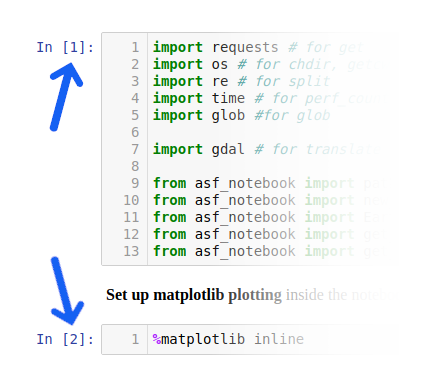
\includegraphics[width=0.7\linewidth]{files/cell_numbers-41fe16375e4710038066a4a0596391c8.png}
\caption*{The cell execution counter indicates the order in which code cells have run.}
\end{figure}

\subparagraph{Run a Single Code Cell}\label{run-a-single-code-cell}

\begin{enumerate}
\item Select the cell you wish to run.
\item Do one of the following:\begin{itemize}
\item Click the \texttt{▶} button at the top of the notebook.
\item \texttt{Ctrl + Enter} or \texttt{Cmd + Enter} (Mac) to run a cell.
\item \texttt{Shift + Enter} to run a cell and select the cell below
\item \texttt{Alt + Enter} to run a cell and insert an empty cell below
\end{itemize}
\end{enumerate}

\subparagraph{Run Multiple Code Cells}\label{Run-Multiple-Code-Cells}

\subparagraph{Run a batch of selected cells}\label{Run-a-batch-of-selected-cells}

\begin{enumerate}
\item Select a group of cells.
\item Do one of the following:\begin{itemize}
\item Click the \texttt{▶} button at the top of the notebook.
\item \texttt{Ctrl + Enter} to run a cell.
\item \texttt{Shift + Enter} to run a cell and select the cell below
\item \texttt{Alt + Enter} to run a cell and insert an empty cell below
\end{itemize}
\end{enumerate}

\subparagraph{Run Every Cell Above or Below a Code Cell}\label{Run-Every-Cell-Above-or-Below-a-Code-Cell}

Select a cell, then:

\begin{itemize}
\item Select the menu option: \texttt{Run} -\textgreater   \texttt{Run All Above Selected Cell}
\item Select the menu option: \texttt{Run} -\textgreater  \texttt{Run Selected Cell and All Below}
\end{itemize}

\subparagraph{Run an Entire Notebook}\label{Run-an-Entire-Notebook}

If you wish to run every code cell in a notebook, you can do one of the following:

\begin{itemize}
\item Select the menu option: \texttt{Run} -\textgreater  \texttt{Run All}
\item Select the menu option: \texttt{Kernel} -\textgreater  \texttt{Restart Kernel and Run All Cells...}
\end{itemize}

\begin{framed}
\textbf{Restarting the Kernel and Rerunning vs. Simply Rerunning}\\
Rerunning a notebook without restarting the kernel preserves previously defined local variables. This can potentially cause issues related to directory changes, paths, and variables containing unexpected values. It is generally safer to restart the kernel and rerun the notebook.
\end{framed}


\bigskip
\centerline{\rule{13cm}{0.4pt}}
\bigskip

\subparagraph{Rerunning a Notebook}\label{rerunning-a-notebook}

We recommend restarting the notebook kernel before rerunning it since any initialized variables and data structures from a previous run persist in memory along with their values, which can lead to unintended results.

To restart the kernel so you can begin a fresh notebook run use one of the following options:

\begin{itemize}
\item Select the menu option: \texttt{Kernel} -\textgreater  \texttt{Restart Kernel}
\item Select the menu option: \texttt{Kernel} -\textgreater  \texttt{Restart Kernel and Clear...}
\end{itemize}

\begin{framed}
\textbf{Clearing Notebook Output}\\
It is easy to lose track of your position in a notebook if it contains code cell output and execution counters from a previous run. We recommend clearing any output before rerunning a notebook.
\end{framed}


\bigskip
\centerline{\rule{13cm}{0.4pt}}
\bigskip

\paragraph{Clearing Cell Output Before Closing}\label{clearing-cell-output-before-closing}

For large notebooks with a lot of plots and images, we recommend clearing all code cell output before closing or saving a notebook. Leaving the output in place can increase the file size of the notebook, which can cause slower notebook loading times (especially if you have a slow internet connection).